% Chapter 1

\section*{\centering Preface}
This chapter gives a brief introduction on batteries and the terms associated with understanding a battery technology. Lithium-ion batteries and its shortcomings are discussed, and a comparison between batteries that currently exist in the market is made. Aluminium-ion batteries, both aqueous and non-aqueous, are introduced and ways of finding new cathode materials that can be used in aluminium-ion batteries is explored.
\newpage
\chapter{Batteries --- an introduction} % Main chapter title
 \label{chap1} % For referencing the chapter elsewhere, use \ref{Chapter1} 
%----------------------------------------------------------------------------------------
% Define some commands to keep the formatting separated from the content 
\newcommand{\keyword}[1]{\textbf{#1}}
\newcommand{\tabhead}[1]{\textbf{#1}}
\newcommand{\code}[1]{\texttt{#1}}
\newcommand{\file}[1]{\texttt{\bfseries#1}}
\newcommand{\option}[1]{\texttt{\itshape#1}}

%----------------------------------------------------------------------------------------
To combat climate change, significant number of steps have been taken to switch over to renewable sources of energy from non-renewables. By installing solar panels on their rooftops, consumers are now powering their houses by tapping solar energy. Figure \ref{Figures/chap1fig:iec} displays the data from 2018 generated by International Energy Association (IEA). However, solar and wind energies have variable output. The sun doesn't always shine and the wind doesn't always blow. Energy storage is necessary for a continuous power supply. Batteries maximize the ability to use the electricity generated by renewable sources of energy, on a day-to-day basis. They store energy in a chemical form, which can be used at a later time. If used in houses, a battery can store the power generated by the sun for several hours. In a grid system, when the supply is higher than demand, electricity can be used to power batteries. When the demand is higher than supply, stored energy can be used by the grid and distributed. To understand how a battery works, it is important to understand a few terms that are helpful in evaluating its performance.  

\begin{figure}[tbh!]
\centering
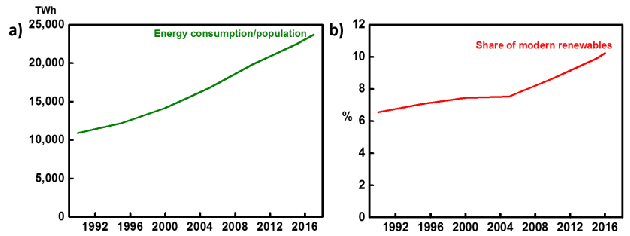
\includegraphics[width=\textwidth]{Figures/chap1fig/iec.pdf}
\caption{Based on International Energy Agency (IEA) data from 2018 monthly oil data service. Significant increase can be seen in recent years in energy consumption and share of modern renewables. This means in spite  of increase in energy consumption, there is also an awareness about using non-renewable sources of energy, www.iea.org/statistics. All rights reserved.}
\label{Figures/chap1fig:iec}
\end{figure}

\begin{itemize}
\item \textbf{Battery capacity}: Capacity is the amount of charge or energy stored in a battery. Mathematically, it is evaluated by integrating current over time. The fundamental units of battery capacity is coulombs (C), though Amp-hrs (Ah) is more commonly used.  Theoretical capacity (the ideal capacity a battery can store under equilibrium conditions) is calculated with the help of chemical reactions that take place inside the cell. Using Faraday's constant (F = 96,484.56 C mol$^{-1}$), theoretical capacity of a battery can be determined using Equation \ref{eq1}:

\begin{equation} \label{eq1}
  \text{Capacity(Ah) = } \frac{n \times F \times 1 \text{ hour}}{3600 \text{ sec}}\\
\end{equation}

where n = number of electrons participating in the chemical reaction \\
F = Faraday's constant. Specific capacity is the capacity stored in a material per unit mass. The most commonly used unit is mAh g$^{-1}$. \\
\item \textbf{Battery potential or voltage}: It is the point (usually in the middle of a discharge curve), where voltage stays constant for the longest period forming a plateau. Various factors such as electrolyte stability, polarization of the battery (displacement of electrode potential from the equilibrium value) and concentrations of the active species help in determining a cell's voltage. Figure \ref{Figures/chap1fig:CDCforcellvoltage} represents a typical charge/ discharge curve. To avoid any permanent damage, a battery should not be discharged below a certain level. This voltage is called the "cut-off voltage". Going beyond the upper or lower cut-off voltages might lead to certain reactions that decompose the electrolyte (also known as side reactions) resulting in an irreversible capacity loss.\\

\begin{figure}[tbh!]
\centering
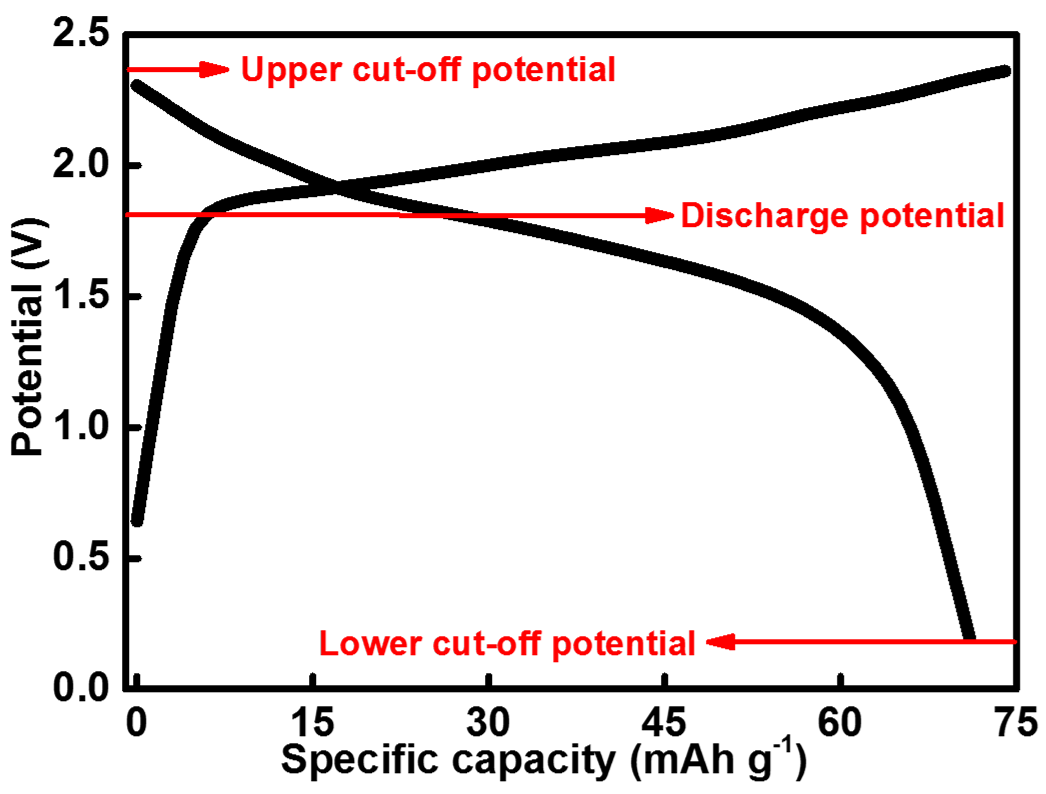
\includegraphics[width=\textwidth]{Figures/chap1fig/CDCforcellvoltage}
\caption{A charge and discharge curve of an aluminium-ion cell using graphite as the cathode and pure aluminium as the anode. The cell was charged and discharged to 2.45 V and 0.2 V respectively. The plateau is observed at 1.75 V, also called nominal voltage.}
\label{Figures/chap1fig:CDCforcellvoltage}
\end{figure}

Sometimes however, a distinct discharge plateau is not observed. In that case, the average potential of the cell is considered to the intersection of the charging and discharging curve, displayed in Figure \ref{Figures/chap1fig:batpot}. 

\begin{figure}[tbh!]
\centering
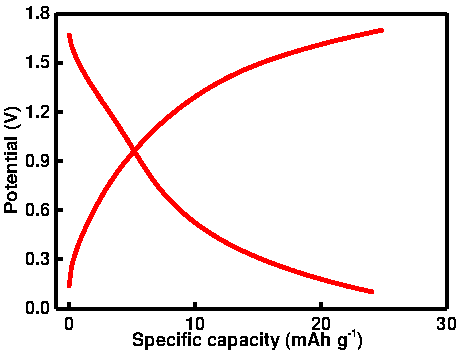
\includegraphics[width=\textwidth]{Figures/chap1fig/batpot.pdf}
\caption{A charge and discharge curve of an aluminium-ion cell using graphite as the cathode and pure aluminium as the anode. The cell was charged and discharged to 2.45 V and 0.2 V respectively.}
\label{Figures/chap1fig:batpot}
\end{figure}

\item \textbf{Energy density}: The amount of energy stored in a battery per unit mass or volume is called its energy density. Sometimes, heavy batteries are required to move something as large as a car over long distances, therefore they use batteries with high energy density. A simple way to determine the specific energy or energy density of a battery is using equation\ref{eq2}:

\begin{equation} \label{eq2}
    \text{Energy density (Wh = } \text{Battery capacity (Ah)} \times \text{Battery voltage (V)}\\
\end{equation}

A higher battery capacity or voltage or both are the prerequisites of a good battery system. The energy densities of all materials tested in this thesis have been reported in Chapter \ref{chap9}.\\

\item \textbf{Power density}: Power density measures how quickly a battery can deliver energy. Also known as specific power, it is equivalent to the maximum current one can draw from a battery. Units used to describe power density are W kg$^{-1}$ or W m$^{-3}$. The best way to differentiate between energy and power density of a battery is to use an example of a moving car. Energy density determines how 'far' the car will go, whereas power density determines how 'fast' the car will go.

\item \textbf{Coulombic efficiency (CE)}: Coulombic efficiency of a battery is the ratio of number of charges that enter during charge to the number that can be extracted from the battery during discharge. A high CE in excess of 95\% is considered a standard value for commercial battery systems. 
\end{itemize}

Batteries can be categorised as primary (non-rechargeable) or secondary (rechargeable). \textbf{Primary} batteries produce current immediately when assembled. Since these battery systems cannot be recharged again, they have high energy densities for one-time use. Common types of primary batteries include zinc-carbon and alkaline batteries. 
\textbf{Secondary} batteries, need to be charged before their first use. They are assembled in the discharged state and applying a charging current reverses the cell's active materials chemical state. They find extensive use in portable devices as they store energy that can be drawn after every charge/discharge cycle. The most commonly used examples of rechargeable batteries are nickel-cadmium (Ni-Cad), nickel metal hydride (NiMH) batteries and lithium-ion batteries (LIBs). \\  
In addition, charging and discharging rates affect the battery capacity. If a high discharge current is applied (i.e. the battery is being discharged very quickly) the amount of energy that can be extracted from the battery is reduced and its capacity decreases. This is because only a fraction of the total reactants are converted to other forms, and therefore the energy available for consumption is reduced. Alternately, if a battery is discharged using low current, more energy can be extracted from the battery and its capacity is higher. The battery temperature also affects the energy that can be extracted. At a higher temperature, the capacity is typically higher than at a lower temperature. However, intentionally elevating battery temperature is not an effective method as this might decrease battery lifetime\cite{leng_effect_2015, ma_temperature_2018}. 
An ideal battery should be low-cost, charge and discharge indefinitely under high or low current rate, have a long lifetime with high CE (>99\%), and experience low-self discharge. However, it is difficult to fulfil all of the above set of requirements. Researchers are building new batteries that might achieve these objectives in their own ways\cite{slater_sodium-ion_2013,jian_carbon_2015,aurbach_prototype_2000,lin_ultrafast_2015}. Every appliance that uses rechargeable batteries has its own specifications. Portable electronic items need faster charging rates, therefore LIBs are extensively used. On the other hand, NiMH and Ni-Cad batteries are cheaper and are used in making electric vehicles. The cost of a hybrid car starts from \$23,000 and a Tesla starts from \$35,000. \\

Table\ref{table1} compares a few characteristics of rechargeable batteries that currently exist in market. 

\begin{sidewaystable}
\centering
\caption{Characteristics of commonly used rechargeable batteries.} \label{table1}
\begin{tabular}{ |p{3.5cm}|p{2cm}|p{2cm}|p{2cm}|p{4.5cm}|p{4.5cm}|}
 \hline 
\textbf{Battery type} & \textbf{In market since} & \textbf{Energy density} & \textbf{Nominal voltage (V)} & \textbf{Applications} & \textbf{Limitations}\\ 
\textbf{} & \textbf{} & \textbf{(Wh kg$^{-1}$)} & \textbf{} & \textbf{} & \textbf{}\\ 
\hline
Lead-acid & 1881 & 30-50 & 2.0 & backup power supplies for telephone and computer centres, grid energy storage, uninterrupted power supply (UPS), marine applications- submarines & Environmental hazard, low energy density, risk of thermal runaway, transportation restrictions\\
Nickel-cadmium (Ni-Cad) & 1960 & 40-80 & 1.2 & portable electronics, toys, cordless telephones & Environmental hazard, low energy density, high self-discharge, explosive\\
Nickel-metal hydride (Ni-MH) & 1990 & 60-120 & 1.2 & Consumer electronics, electric vehicles, hybrid cars & Expensive, high self-discharge, high maintenance\\
Lithium-ion (\ce{LiCoO2}) & 1991 & 150-190 & 3.6 & Smartphones, laptops, tablets, digital cameras, hybrid vehicles, electric motorcycles, scooters, bicycles, personal transporters & Safety hazard, risk of thermal runaway, transport restrictions, environmental hazard\\
Lithium-ion (\ce{LiMn2O4}) & 1996 & 100-135 & 3.8 & Same as above & Same as above\\
Lithium-ion (\ce{LiFePO4}) & 1999 & 90-120 & 3.3 & Same as above & Same as above\\
Lithium-ion (LiNi$_{x}$Co{$_{1-x-y}$}O$_{2}$, LiNMC) & 2008 & 190-210 & 3.6 & Same as above & Same as above\\
\hline
\end{tabular}
\end{sidewaystable}

\newpage

\section{Lithium-ion battery (LIB)}
The standard potentials of a pair of half reactions reaction determines whether a voltage is generated in a redox reaction or not. If the difference between standard potentials is positive, then the reaction will proceed spontaneously, which is precisely what is needed in a battery. Therefore, standard potential is an important parameter while finding a suitable battery anode\cite{liu_understanding_2016}. Out of all the metals that can be used in a battery system listed in Table \ref{table2}, Lithium has the most negative standard reduction potential (-3.04 V), which enables it to achieve very high energy and power densities when paired with many different materials (refer to equation \ref{eq2}). This is the reason why LIBs are a popular battery-choice for most applications.
\subsection*{Mechanism of a lithium-ion battery}
The cathode typically consists of lithium-cobalt oxide \ce{LiCoO2} or lithium iron phosphate \ce{LiFePO4}. The anode is generally made from graphite and the electrolyte varies from one type of lithium battery to another. All LIBs have a similar working principle. During charging process, the two electrodes are connected externally to an external electrical supply. The electrons are forced to be released at the cathode and move externally to the anode. Simultaneously the lithium ions move in the same direction, but internally, from cathode to anode via the electrolyte. In this way the external energy are electrochemically stored in the battery in the form of chemical energy in the anode and cathode materials with different chemical potentials. The opposite occurs during discharging process: electrons move from anode to the cathode through the external load to do the work and Li ions move from anode to the cathode in the electrolyte. This is also known as \enquote{shuttle chair} mechanism, where the \ce{Li+} ions shuttle between the anode and cathodes during charge and discharge cycles. Electrochemical reactions at the two electrodes release the stored chemical energy \cite{deng_li-ion_2015}. The overall reaction during discharge is given below. The equation is reversed during charge. 

\begin{align}
    \ce{CoO2} + \ce{LiC6} \longrightarrow \ce{LiCoO2} + \ce{C6}
\end{align}

\vspace{3mm}

A lithium-based battery is a power pack of choice not only on the Earth, but also in space. In October 2019, a few astronauts on board the International Space Station (ISS) stepped outside their quarters for a spacewalk. Flight engineers Christina Koch and Jessica Meir were assigned the task of manually swapping out two nickel hydrogen (NiH) batteries for one brand new LIB. It was also the first ever all-female spacewalk in human history! The battery replacement would not only upgrade the station's electrical system but also extend it's life, at least through 2020's. ISS was launched into orbit in 1998 with 48 NiH batteries. The National Aeronautics and Space Administration (NASA) has started swapping these old batteries, since 2017, with 24 new LIBs  that provide higher energy density and a better power efficiency. Naturally, they had to be careful while handling these heavy batteries (195 kg). LIBs come with a potential risk of thermal runaway, which means an increase in temperature leads to conditions that cause a further increase in temperature inside the batteries, often leading to destructive results. Inside a pressurised oxygen-rich capsule, that would have been catastrophic.\\
An electrolyte is a chemical medium that allows the flow of charge between the cathode and anode. It promotes movement of ions from the cathode to the anode. It is usually made of soluble salts, acids or other bases in liquid, gelled or dry media, a polymer, or ionic liquids (ILs), also known as molten salts \cite{xu_nonaqueous_2004,armand_ionic-liquid_2009,croce_nanocomposite_1998}. The ions transport current through the electrolyte, while the electrons flow in the external circuit generating an electric current. LIBs use lithium hexafluorophosphate (\ce{LiPF6}) and mixture of carbonate solvents such as dimethyl carbonate (DMC), ethyl methyl carbonate (EMC), or diethyl carbonate (DEC) as electrolytes. They are less viscous electrolyte and enhance its conductivity. However, they are flammable and show flash points around room temperature (between 16 and 33$^{\circ}$C). In combination with an oxidant and an ignition source, they may catch fire and cause explosions! In addition, future battery demand will place increasing pressure on lithium and cobalt reserves\cite{turcheniuk_ten_2018}. To find a suitable alternative, one needs to examine theoretical specific capacities of different ions that can replace lithium. Metals in the upper left corner of the periodic table, such as sodium (Na), magnesium (Mg), potassium (K) and calcium (Ca) report higher theoretical capacities than other metals and can be alternatively used as battery anodes. Table  \ref{table2} compares the metrics of a few potential metal anodes including aluminium. With three-electron redox properties (\ce{Al3+}/Al) has high specific capacity per mass unit (2980 A h kg$^{-1}$) and the highest capacity per unit of volume (8046 A h L$^{-1}$)\cite{ambroz_trends_2017}.

\begin{table}[tbh!]
\caption{Comparing important parameters of various metal anodes.} \label{table2}
\begin{tabular}{|ccccccc|}
\hline
 & \textbf{Li} & \textbf{Na} & \textbf{Mg} & \textbf{Al} & \textbf{K} & \textbf{Ca}\\
\hline
\hline
Valence electrons & 1 & 1 & 2 & 3 & 1 & 2\\
Specific capacity (mAh g$^{-1}$) & 3862 & 1166 & 2205 & 2980 & 685 & 1340\\
Standard potential (V) & -3.04 & -2.71 & -2.36  & -1.68 & -2.93 & -2.87\\
Crustal abundance (ppm) & 18 & 22700 & 23000 & 82000 & 18400 & 41000\\
\hline  % Please only put a hline at the end of the table
\end{tabular}
\end{table}

High abundance and easy accessibility of aluminium resources enable aluminium-ion batteries (AIBs), together with their electrochemical characteristics, offer an opportunity to become the ideal alternative.

\section{Aluminium-ion battery (AIB)}
The second most promising metal despite having a higher standard oxidation potential than lithium, is aluminium (Al). AIBs use aluminium metal as anode, which makes it cost-effective, recyclable, and environment-friendly. Due to the presence of three electrons in its valence shell that can easily participate in the electron transfer process, a multi-electron reaction is feasible, which increases its theoretical energy density (Table \ref{table2}). Moreover, the high crustal abundance and easy accessibility of aluminium resources enable AIBs to become an ideal candidate for large-scale energy storage systems. \\
The idea to use aluminum in batteries was born in 1800's. Inventors like Joseph Richards and James Sully worked on galvanic batteries using a carbon-aluminum electrode \cite{noauthor_james_1897,richards_aluminium_1890}. These cells maintained a nearly constant electromotive force (EMF) on closed circuit for several weeks at a time. The negative electrode was externally exposed to air and a mixture of potassium carbonate (\ce{K2CO3}) and kerosene oil was used as the electrolyte. Their motive was to provide an aluminum dry cell with a longer shelf life. Another attempt was made to make commercially viable aluminium batteries in the 1950's. Donald Sargent reported an Al/NaOH and ZnO/\ce{MnO2} system . Both these systems suffered through similar problems of formation of a layer of aluminium oxide, also known as \enquote{passivation}, leading to very low energy densities and hence could not be commercialised. Aluminium– air batteries (Al–air batteries) produce electricity from the reaction of oxygen in the air with aluminium. The cathode is immersed in a water-based electrolyte (alkali metal salts) and forms hydrated \ce{Al2O3}. Once the Al anode is consumed by its reaction with atmospheric \ce{O2} at a cathode, the battery dies. One of the first aluminium- air batteries were reported by Zaromb\cite{zaromb_use_1962} in the 1960s. He found that addition of zinc oxide or ammonium salts to the electrolyte reduced the rate of aluminum corrosion in the strongly basic electrolytes. However, the nature of the stabilization was irregular and sometimes the corrosion rate would experience a sudden increase\cite{bockstie_control_1963}. In 2002, Li \textit{et al.} discovered the reversible electrodeposition of aluminum from both aqueous and non-aqueous electrolytes\cite{li_aluminum_2002}. This showed that aluminum might be used as an anode in rechargeable batteries. However, the passivating oxide layer on the anode surface was still a matter of concern and was continuously deteriorating the battery performance. The passivation caused a decrease in the electrode potential resulting in lower cell voltages than the expected theoretical value. The oxide layer further inhibited the cell performance by causing a \enquote{delayed action}, which is a time delay during which the cell reaches its operating voltage during discharge. This delay was due to the gradual breakdown and removal of the oxide layer from the aluminum anode surface, which also affected the anode activation. Finally in 2010, Paranthaman \textit{et al.} made the first rechargeable aluminum-ion battery using a cathode composed of \ce{Mn2O4} and an ionic liquid (IL) as the electrolyte, based on the works by Jiang \textit{et al.} and Peng \textit{et al.} \cite{paranthaman_transformational_2010, jiang_electrodeposition_2006,peng_investigation_2008}. 
The electrolyte was made of aluminium trichloride (\ce{AlCl3}) and 1-Ethyl-3-methylimidazolium chloride (EMImCl) (discovered by Gillford \textit{et al.}) in a ratio of 2:1 \cite{gifford_aluminum/chlorine_1988}. The higher concentration of \ce{AlCl3} makes the IL a Lewis acid, which prevented Al passivation. 
Reversible deposition and dissolution of Al occurs in non-aqueous electrolytes such as molten salts NaCl-\ce{AlCl3} or ILs (quaternary ammonium species) at room temperature with no passive oxide layer being formed on the aluminum anode \cite{vestergaard_molten_1993,galinski_ionic_2006,elia_insights_2017}. The stability of the ILs within the electrochemical window prevented side reactions and enabled deposition of Al, which increased the cell voltages \cite{li_aluminum_2002}.\\ ILs consist of weakly coordinated complex ions, which are liquid below 100 $^{\circ}$C, or at room temperature \cite{hayes_structure_2015}. Another advantage of the ILs is their wide electrochemical window, ranging from 4.5 to 6.0 V. This makes them suitable for high-performance energy storage devices \cite{wang_binder-free_2015}. In addition, most ILs show a high thermal stability, non-flammability, non-volatility and a zero vapor pressure, in comparison to organic solvents \cite{dieter}. Cations such as 1-ethyl-3-methylimidazolium (EMIm), 1,3-di-nbutylimidazolium or 1-butylpyridinium (Figure \ref{Figures/chap1fig:cations}), in combination with chloroaluminate (Al$_x$Cl$_y$) anions can achieve a potential window of up to 6 V. Furthermore, they reach an electric conductivity of 10 mS cm$^{-1}$, which is similar to the magnitude of most aqueous electrolytes \cite{ngo_thermal_2000}. ILs based on \ce{AlCl3} are mostly hygroscopic \cite{ueda_electroplating_2012}. A tiny amount of moisture might decompose them or decrease its voltage window. The Lewis acidity of chloroaluminate-based ILs depends on the molar composition of the anion and cation components, which also affects their conductivity and viscosity \cite{buzzeo_non-haloaluminate_2004}. 
Al deposition (during charge) and dissolution (during discharge) at the anode takes place in a Lewis acidic IL, containing \ce{Al2Cl7}$^-$ (equation \ref{eq3} \cite{galinski_ionic_2006}.

\begin{figure}[tbh!]
\centering

\includegraphics[width=\textwidth]{Figures/chap1fig/cations}
\caption{Schematic illustration of the molecular structure of cations from the room temperature ionic liquids (ILs) used for rechargeable batteries. a) 1-ethyl-3-methylimidazolium cation, b) 1-butyl-3-methylimidazolium cation and c)1-butylpyridinium cation.}
\label{Figures/chap1fig:cations}
\end{figure}

\begin{align} \label{eq3}
   4\ce{Al2Cl7^{-}} + 3\ce{e-} \rightleftharpoons \ce{Al} + 7\ce{AlCl4^{-}}  
\end{align}

\ce{Al2Cl7}$^-$ anions are formed when the molar ratio of \ce{AlCl3} is higher than 0.5, the IL becomes a Lewis acid. An excess of the cation results in an IL, which is a Lewis base, due to the presence of free halide ions (Equation \ref{eq4}) \cite{holbrey_ionic_1999}. A neutral composition consist of the same molar ratio of \ce{AlCl3} and EMImCl. 

\begin{align}\label{eq4}
   2\ce{AlCl4^{-}} \rightleftharpoons \ce{Al2Cl7-}+\ce{Cl-} 
\end{align}

Using \ce{AlCl3}/EMImCl electrolyte in AIBs was a major breakthrough since most of the earlier inventions displayed lower capacity and were not good enough for long term practical use. EMImCl/ \ce{AlCl3} has since been the most commonly used electrolyte for non-aqueous aluminum-ion batteries.
% This was the reason why aluminium batteries were never good enough for long-term practical use. Holleck and Giner studied the electrochemistry of aluminum metal in the \ce{AlCl3}-KCl-NaCl eutectic melt as a possible electrolyte for aluminum batteries with high energy densities. They also found that the aluminum anode was passivated in these melts by formation of a solid salt layer due to local concentration changes at the metal surface during current flow. In addition, the cathodic deposition of aluminum resulted in formation of dendrites and production of chlorine gas\cite{holleck}. The oxide layer of an aluminum anode caused a number of problems preventing these cells from commercialisation. 
Figure \ref{Figures/chap1fig:AIBmech} illustrates an AIB using an IL  (made EMImCl/\ce{AlCl3}) electrolyte and 99\% pure Al foil as anode and a cathode with a layered structure. 

\begin{figure}[tbh!]
\centering
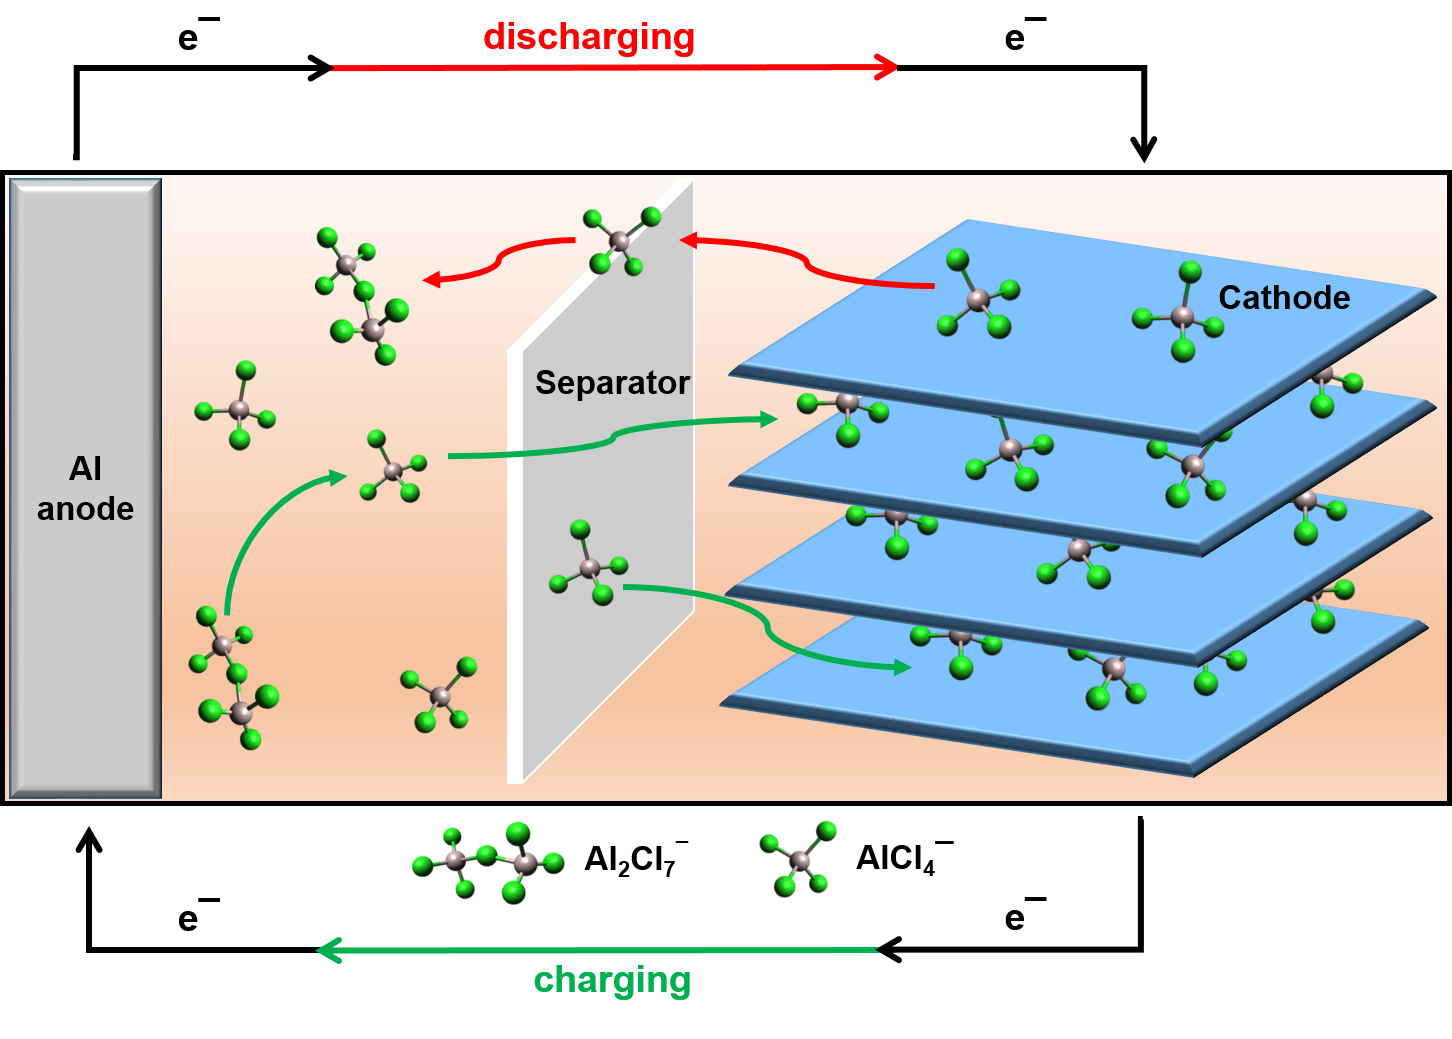
\includegraphics[width=\textwidth]{Figures/chap1fig/AIBmech}
\caption{A schematic representation of a non-aqueous aluminium-ion battery (AIB).}
\label{Figures/chap1fig:AIBmech}
\end{figure}

Based on the type of electrolyte used, AIBs can be categorised as aqueous AIBs and non-aqueous AIBS.  

\subsection{Aqueous aluminium-ion batteries (AAIBs)}
Using water as an electrolyte would reduce the battery costs significantly and increase battery safety. However, these batteries have their own set of problems. 

\begin{itemize}
    \item the electrochemical plating/stripping of aluminium occurs during charge and discharge cycles at a voltage far from the stable voltage window of water, which means unnecessary side reactions such as water splitting are bound to occur
    \item aluminium trichloride \ce{AlCl3} when used without ILs is highly acidic and might result in dissolution of active material leading to corrosion of battery parts
    \item a cathode material with a good cycling stability is yet to be discovered
\end{itemize}  

Improving characteristics such as cycle life, efficiency and rate capability would enable these batteries to be used for high power applications. However, limited focus has been given to cycle life, efficiency and rate capability in the recent aqueous Al-ion literature. Anatase titanium oxide (\ce{TiO2}) has been investigated as an intercalation electrode for AAIBs and \ce{TiO2} nanostructures have been commonly used. Cycling data for \ce{TiO2} nanotubes were presented up to cycle 13 by Liu et al \cite{liu_aluminum_2012}.  %Recently, a graphene enhanced \ce{TiO2} electrode was shown to produce a capacity between 10 and 25 mAh g$^{-1}$ at a current density of 6.25 A g$^{-1}$. However, only 125 cycles were possible and coulombic efficiency was observed to be very low at approximately 50\%. Similarly, the charge discharge profiles observed for the nanospheres and nanotubes show low coulombic efficiencies of around 80-85\%. The reason for low efficiency of \ce{TiO2} in aqueous AIB electrolyte is yet to be explored, but the possibilities could be oxidation of \ce{Ti3+} due to dissolved \ce{O2} in electrolyte, \ce{H2} gas evolution or an irreversible reduction of \ce{Ti4+} to \ce{Ti2+} while charge.  
Aluminium in aqueous systems instantaneously forms a very thin (thickness $\sim$2-10 nm) surface layer of \ce{Al2O3} \cite{vargel_corrosion_2004}. This layer is quite stable over a pH range of about 4.0-8.6. Electrode passivation might prove advantageous in LIBs, but it creates a barrier for dissolution of Al anode and transportation of \ce{Al^{3+}} ions \cite{myung_electrochemical_2011}. For this reason, AAIBs fail to achieve high energy densities and long cycle lives for long-term practical uses.

\subsection{Non-aqueous AIBs}
As discussed in Section 1.2, chloroaluminates (Al$_x$Cl$_y$) have been known for aluminium electrodeposition since the 1970s and are now being used as electrolytes for non-aqueous rechargeable aluminium batteries\cite{weppner_ionic_1976, fung_reaction_1972}. Systems with a general formula MCl-\ce{AlCl3} where \ce{M+} can be a cation like \ce{Na+}, \ce{Li+} or an organic species like pyrrolidinium or imidazolium have been tested as electrolytes for rechargeable AIBs\cite{das_aluminium-ion_2017}. These melts can be acidic, basic or neutral. In the acidic systems, the dominant species is \ce{Al2Cl7^{-}}, while in a basic system \ce{Cl-} and \ce{AlCl4^{-}} anions coexist whereas in neutral melts, only \ce{AlCl4-} anions exist \cite{galinski_ionic_2006,holbrey_ionic_1999}. Since the standard electrode potential of \ce{Al^3+}/Al at -1.68 V is lower than \ce{H+}/\ce{H2}, evolution of \ce{H2} gas occurs when Al foil reacts with aqueous acid or alkali solution. Thus, Al is unable to undergo electrochemical stripping or deposition in a common aqueous solution \cite{wu_electrochemically_2019}. To be compatible with Al anode, the IL \ce{AlCl3}/EMImCl emerges as the typical electrolyte. It provides a mild corrosive effect on the anode surface to activate the Al striping and plating reaction. The equation below describes the reaction that takes place between the anode and the IL. During the discharge, Al is oxidized to form \ce{Al3+} ions. These ions move to the cathode together with the coordination anions from the electrolyte (\ce{AlCl4-} and \ce{Al2Cl7-}) and intercalate into the material. When the battery is recharged, the redox reactions are reversed.

In 2017, Kravchyk and his group emphasized that an \ce{AlCl3} graphite battery does not have a \enquote{rocking-chair} mechanism. The group claimed that these systems should not be called an \enquote{Al-ion batteries} because the species that reversibly intercalate into the graphitic cathode (\ce{AlCl4-}) are different from the ions involved in the deposition and stripping of Al atoms and/or \ce{Al^3+} ions from the aluminium foil. They showed that \ce{AlCl3} acts as the anode during the charging process, and gets reduced to Al atoms for electrodeposition and simultaneously generates \ce{AlCl4^-} for intercalation. They proposed that the ionic liquid, in fact, acts as a capacity-limiting liquid anode and not just as an electrolyte.

\begin{align*}
        \ce{Al} + 7x\ce{AlCl4-} \rightleftharpoons 4x\ce{Al2Cl7-} + 3x\ce{e-}
\end{align*}

The ILs not only overcome the above-mentioned problems with AAIBs, \ce{AlCl3}/ imidazolium is the quintessential electrolyte for non-aqueous AIBs making them much safer than LIBs \cite{jayaprakash_rechargeable_2011, lin_ultrafast_2015,wang_new_2013-1,rani_fluorinated_2013}. 

\section{Cathodes for rechargeable batteries}
A usable cathode material should have certain properties: good conductivity, stability in the presence of an electrolyte, good working voltage and a large reversible storage capacity obtainable at that voltage and high natural abundance. In addition, it should be easy to fabricate. Theoretical capacity of a cathode material (C$_{t}$) can be found using equation:

\begin{equation} \label{eq5}
   C_{t} \text{ = } \frac{n \times F}{3.6 \times M}
\end{equation}\\
where n = number of reactive electrons per formula unit,\\
M = molar weight of the cathode material and\\
F = Faraday constant\\
Equation \ref{eq5} implies that a material with a low molecular weight and high number of reactive electrons would deliver a high theoretical capacity.

\begin{figure}[h!]
\centering
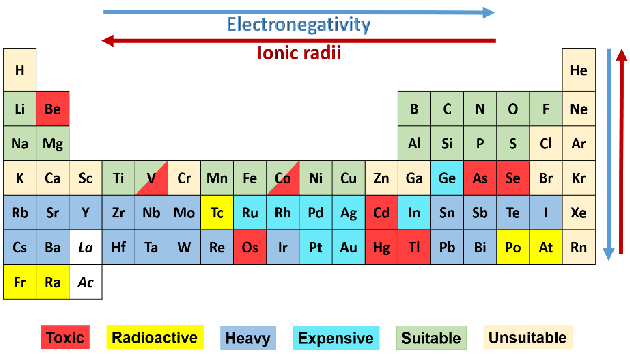
\includegraphics[width=\textwidth]{Figures/chap1fig/pertab.pdf}
\caption{The periodic table suggesting elements that can be used as battery materials. However, a few elements from this table have shown good electrochemical performance such as Mo, Sn, Nb and W. Potassium and calcium-ion batteries have also been studied.}
\label{Figures/chap1fig:pertab}
\end{figure}

A perfect battery that works for every application does not exist. It is important to identify the correct battery metrics while selecting a battery for a particular application. For example, a lead-acid battery works great in an automotive starter battery where it provides the required high rate capability. However, with its toxicity and low energy density it would not be suitable for portable electronics. Similarly, not all elements in the periodic table that may provide high energy density, be commercialised for everyday use. Figure \ref{Figures/chap1fig:pertab} displays the elements that can be used for designing new cathodes. Radioactive elements, heavy metals, and inert gases are some of the elements from the periodic table that should never find any long-term practical use in battery applications. Transition metals have variable valence states, which increases the number of electrons that can be stored, increasing the battery capacity. Some transition metals such as vanadium (V) and cobalt (Co), are being used as cathode materials in LIBs despite their toxic nature \cite{cui_carbon/titanium_2010,qu_vanadium_2019,salunkhe_direct_2014,spreafico_pvdf_2014}. Carbon is one of the cheapest materials that has the ability to store large amount of energy \cite{candelaria}. This is one of the reasons why carbon-based materials are the premium choice in any energy storage device.
%The type of bond formed between a metal ion and the ligand plays an important role in determining the electrochemical potential of the material. When the electronegativity difference between the two is high, an ionic bond is formed. A smaller difference results in a covalent bond. Materials with a covalent bonds form poorly packed structures, while ionic bonds form dense structures. A stable structure would enhances the phase stability and electrochemical potential of the material \cite{melot_design_2013}. Furthermore, electrode potential depends on the ionic radius of the material. When an atomic nuclei is loosely bound to its valence electrons, the system needs lower energy for electron transfer , which leads to a lower potential. If more energy is consumed during electron transfer  for materials having a lower ionic radii, the electrochemical potential of the material increases. 
The cell potential \textbf{E} associated with an electrochemical reaction is defined as the decrease in the Gibbs free energy, \textbf{G}, per coulomb of charge transferred and leads to Equation \ref{eq6}, which is derived from the Nernst equation.  :
\begin{equation} \label{eq6}
    \Delta G \text{ = } -nFE
\end{equation}\\
where $\Delta$G = change in internal energy during ion intercalation,\\
n = number of electrons taking part in the redox process,\\
F = Faraday constant and\\
E = electrochemical potential of the material. \\
Liu \textit{et al.} showed that the electrochemical potential of a material is affected by interaction between the atoms or electrons and those interactions also change the internal energy \cite{liu_understanding_2016}. Using polyanionic ligands such as phosphates, sulfates and silicates, which are more electronegative, results in formation of bonds with increased ionic character \cite{liu_understanding_2016}. This further enhances the electrochemical potential of a material \cite{melot_design_2013}. For example, \ce{LiCoPO4} (polyanionic) displays a higher potential at 4.8 V than \ce{LiCoO2} (oxide), which has a potential at 4.0 V\cite{masquelier_polyanionic_2013}. 

\subsection{Cathodes for non-aqueous AIBs}
Based on the material type and structure, cathodes tested during the PhD were mainly categorised into two families.\\
\textbf{Carbon-based materials}: Graphite, a form of carbon with hexagonal structure, has been commonly used as an electrode in various battery systems \cite{xu_charge-transfer_2007,zhang_novel_2016,wu_carbon_2003,jian_carbon_2015}. Its layered structure allows insertion of ions and it also has good thermal and electrical conductivity, and a high electrical potential \textit{vs.} \ce{Al}/\ce{Al^{3+}} of 2.1 V. In graphite-based batteries, Al$_x$Cl$_y$ anions intercalate into the graphitic layers when the cell is being charged and deintercalate during discharge. Electroplating and dissolution of Al takes place at the anode. Figure \ref{Figures/chap1fig:AIBmech} displays the intercalation mechanism, very much similar to LIBs. Different forms of graphite have been used in AIBs. An AIB using graphene nanoribbons on highly porous three-dimensional (3D) graphene foam as cathode exhibited low charging voltage plateaus (cutoff voltage of 2.3 V, below which the battery has no side reactions), high discharge voltage plateaus near 2 V, high capacity about 123 mAh g$^{-1}$ at a current density of 5000 mA g$^{-1}$ with CE higher than 98\% for 10000 cycles at various current rates \cite{yu_graphene_2017}. Fluorinated graphite \cite{rani_fluorinated_2013}, kish graphite flakes \cite{wang_kish_2017}, 3D graphitic-foam \cite{wu_3d_2016}, graphene aerogels\cite{huang_graphene_2019} and several other forms have been tested, which showed discharge capacities ranging from 60-250 mAh g$^{-1}$. \\
Activated carbon, owing to its highly porous structure, provides a high surface area and renders an additional capacitor-like charge storage, where absorption of electrolyte ions takes place on the cathode's surface \cite{eliad_ion_2001, zhu_carbon-based_2011}.\\

The second type of cathode materials are \textbf{two-dimensional (2D) materials} such as transition metal dichalcogenides (TMDs), transition metal oxides (TMOs), MXenes, and a few other metallic oxides. These materials offer tunable chemical and physical properties due to their various elemental compositions and different crystallographic structures. In addition, they possess excellent electrochemical properties \cite{chia_electrochemistry_2015}. A 2D plane imparts a high surface area, which allows complete utilization of all available sites in a cathode material \cite{jia_interfacial_2016,naguib_mxene_2012}.\\ Each metal in a TMD is coordinated with two chalcogens; the metal is in +4 oxidation state while the chalcogen atom is in -2 state. Interaction or insertion of ions from the electrolyte alters the oxidation states of the molecules resulting in redox process. In addition, a few TMDs, especially molybdenum (Mo) and tungsten (W) dichalcogenides, are capable of phase transition after ion insertion (discussed in Chapter \ref{chap4}). Due to introduction of extra electrons and rearrangement of d orbitals, a phase transition from 2H to 1T takes place \cite{acerce_metallic_2015-1}. This changes the electronic properties of the material since 2H \ce{MoS2} is semiconducting, while 1T \ce{MoS2} is metallic. For the above-mentioned reasons, 2D materials have gained enormous attention in recent years. Prussian blue, an organic dye was also tested as a cathode due to its three-dimensional framework and that it should allow insertion of the chloroaluminates. 
%These materials have promoted a relatively reversible trivalent reaction. Strong electrostatic nature of trivalent \ce{Al^{3+}} sometimes leads to sluggish kinetics, high over-potentials, and degradation of the host structure. Therefore, to accommodate the highly charged ions, it is essential for the cathode materials to possess weak bond strengths between the host frameworks. Our unpublished, preliminary density functional theory (DFT) calculations indicated a significant decrease in inter-layer spacing of these materials when \ce{Al^{3+}} cations were assumed to intercalate (owing to the very high charge density of \ce{Al^{3+}}). Therefore, we propose intercalation of \ce{AlCl4-} anions into the layered cathode. XRD, Raman spectroscopy and XPS were used to verify our hypothesis.
During this study, various carbon-based and 2D materials were tested as potential cathodes for rechargeable non-aqueous AIBs. The results have been reported in the subsequent chapters.

\section{Research objectives}
The goal of this PhD project is to find new cathodes for rechargeable AIBs that perform better than state-of-the-art. 
\begin{itemize}
    \item Molybdenum dichalcogenides, a few transition metal oxides or sulfides, boron nitride (inorganic graphite) should undergo an intercalation mechanism to store charge and deliver a stable cycle life with improved specific discharge capacities. 
    
    \item Materials with high surface area such as activated carbon or nanostructured materials, provide a better contact between the cathode and the electrolyte, and prove to be good battery materials \cite{li_commercial_2018,satish_macroporous_2015,banerjee_mof-derived_2014,elazari_sulfur-impregnated_2011,shen_novel_2012}. They provide a faster and an efficient pathway for electron diffusion, which improves the kinetics of the system and increases the battery's energy density. To confirm the above- mentioned hypothesis, high surface-area materials such as activated carbon were synthesised and a few others such as nanostructures of molybdenum dichalcogenides, carbon black from Super-P, electrospun \ce{SnO2} fibres, Prussian blue,etc. were obtained from sources and collaborators and tested as cathodes for non-aqueous AIBs.
    
    \item Once a cathode achieves high capacity (> 60 mAh g$^{-1}$), and a high voltage (> 1.0 V), it is equally important to establish its mechanism. This would help further improve its performance by designing a better cathode. X-ray diffraction studies, Raman spectroscopy, and X-ray photoelectron spectroscopy were a few analytical tools implemented to analyse cathode materials. 

\end{itemize}






